% Modelo de Domínio

Uma primeira fase de desenvolvimento passa pela modelação do domínio do problema, a modo de gradualmente ser modelado o diagrama de classes. Assim sendo, para modelar o domínio, é  necessário ter em conta:
\begin{itemize}
    \item As várias entidades do problema;
    \item Os relacionamento entre as várias entidades, isto é, especificar os termos que envolvem a relação e a cardinalidade associada;
\end{itemize}

As \textit{constrains}, \textit{stakeholders} e objetos a considerar no sistema foram sendo registados ao longo da contextualização e da análise requisitos conforme descrito na secção \ref{sec:requisitos}. A própria esquematização do modelo permite raciocinar sobre a natureza do sistema, e permite isolar num único esquema várias regras de negócio a considerar. Como tal, durante a modelação do domínio surge um produto que permite, por um lado, que a equipa consiga interiorizar especificamente o tipo de sistema a desenvolver e, por outro lado, existe uma maquete que facilita a validação e desenvolvimento de diagramas que se seguem.

\begin{landscape}
    \begin{figure}[!ht]
        \centering
        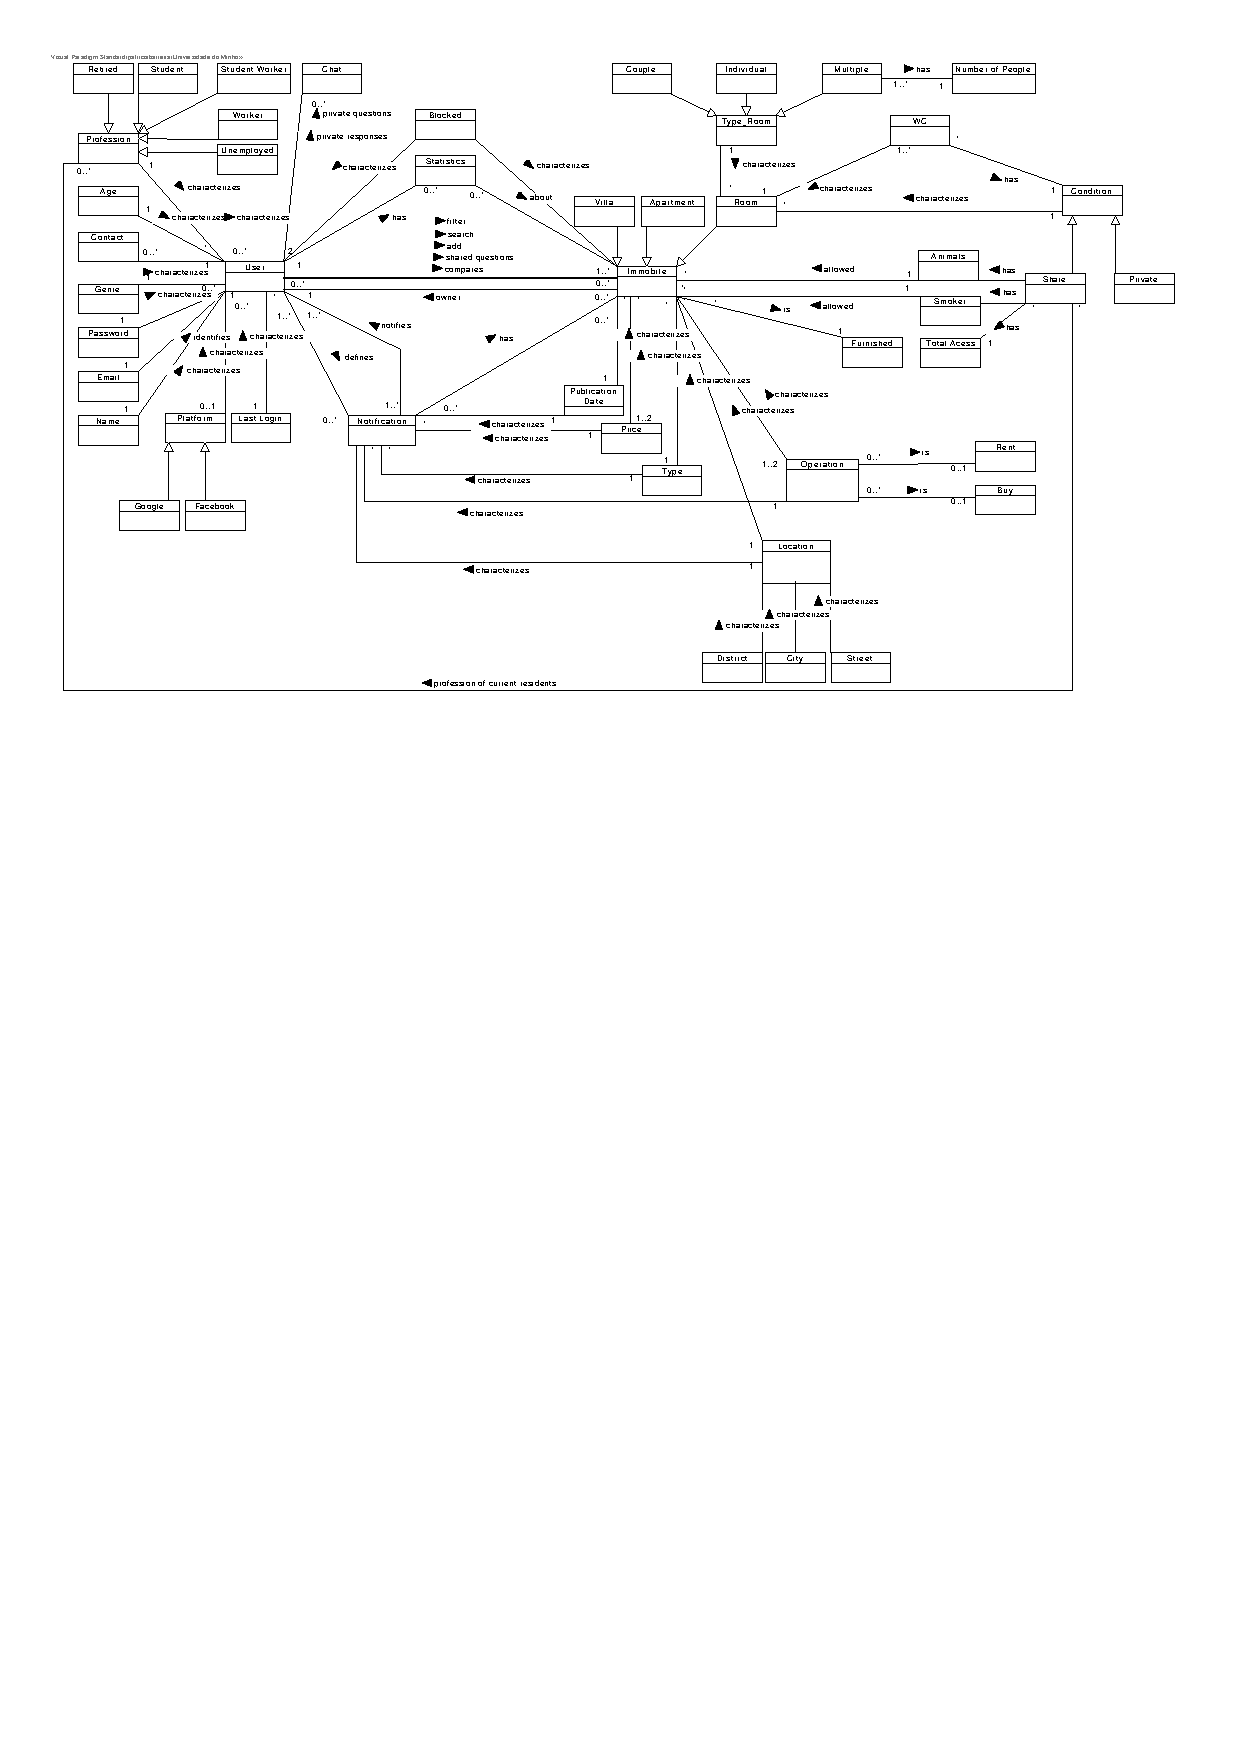
\includegraphics[width=1.8\textwidth]{images/Home4AllDominio.pdf}
        \caption{Diagrama de domínio da aplicação \texttt{Home4All}.}
        \label{fig:diagrama_dominio}
    \end{figure}    
\end{landscape}
